%!TEX root = ../dokumentation.tex

\chapter{Result}

\section{Possibilities to deploy Wildfire post-groomer on Kubernetes cluster}

In chapter 3.3. has been described how a special Wildfire version could be run on Kubernetes. Because of some Spark 2.0.2 dependencies and no native support for Kubernetes in that version this was only possible through a workaround. The success of this solution will be explained in following chapter.

For measuring the success of this solution, first have to be defined, how a success can be recognized. One step for this is of course if the spark submit can be executed in general. A second step would be if a performance increasement can be measured when connecting more worker nodes. Thereby can be determined, if the execution runs in the cluster or just local.

First the execution of the specialized spark submit worked all fine and a result has been printed out at the end. The time for the tested post-groomer station fluctuated between 14 and 16 seconds for a dataset with 50 files with 100000 rows each, so 1.5 Megabyte. This means that the execution was successful in first step, because with that method it is possible to run the spark submit execution on the master node with the in chapter 3.3. specified command.

\begin{figure}[b]
\centering
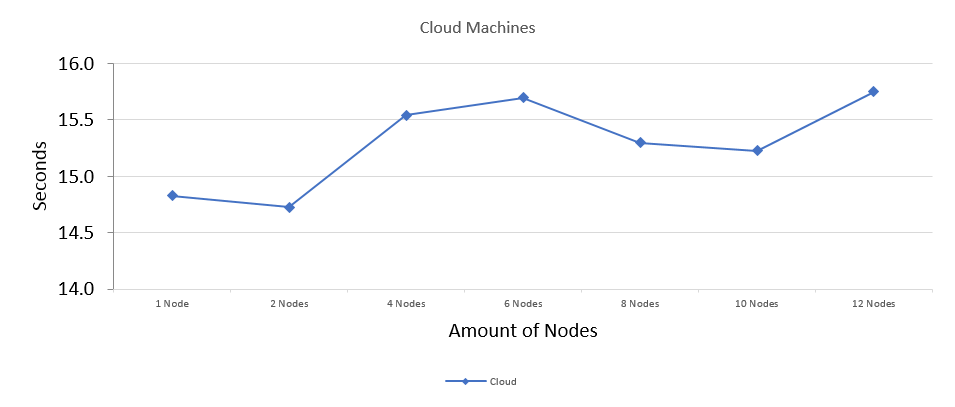
\includegraphics[width=\textwidth/5*4]{images/workaround_testing_results.png}
\textsuperscript{Figure 4.1.1 Testing results of Spark 2.0.2 workaround}
\end{figure}

In second step there had to be run automated tests with different amounts of nodes to test the behaviour of that solution in different environments. Therefore the master node was given 12GB of memory and 12 cores while all the worker nodes were given 8GB of memory and 8 cores. Figure 4.1.1. shows the result of those tests.

This shows, that there is no visible pattern of increasing performance, which can have two reasons: First the used dataset could just be to small to measure performance changes. But second it could also not use the other nodes and run the execution just on the master node.

Therefore the performance of a 12GB and 12 core single node has been compared to a 8GB and 8 core node. Last one has then be used as a master node and two more 8GB and 8 core nodes has been connected to its cluster. The tests showed, that every execution on the 12GB and 12 core node resulted in a time measurement of about 13.95 seconds, while the tests on the 8GB and 8 core node all needed about 19.93 seconds for the post-groomer station. This time didn't change when connecting other nodes to its cluster, which means, that the execution only uses the local resources of the node, on which the command was executed.

Another indication was, that there are no spawning pods observable on the cluster while executing the specified spark submit command. This could have also be caused by the workaround only working in its isolated pods and not publicly showing new spawned pods, but all together it is very probable, that the execution only uses local resources.

This means that the test to run Spark 2.0.2 based operations on Kubernetes failed and the Wildfire version needs to clear all their Spark 2.0.2 dependencies and run on Spark 2.3.0 only to get it runnable on Kubernetes. After it it should be possible to run this version the way described in Listing 3.22 with using ``k8s://https://<master-url>:<master-url-port>'' as master parameter instead of the ``spark://spark-master:7077''.

\section{Results of performance tests}

Besides the evaluation of possibilities to deploy Wildfire post-groomer on a Kubernetes cluster, also the performance of the cloud divices should be compared to physical devices called ``Loud''.

Therefore there had to be run tests in two different environments: First the cloud devices on the one hand, which could be take over by the automated testing script, and second on physical devices. To test it with different specifications the memory and the cores should vary. That's why there had to be several Cloud machines with different specifications. The physical devices could only be limited by parameters in the spark submit command, which limits the used memory and cores for its execution.

Those tests had been run again with a dataset of 50 files with 100000 rows each. Totally that are 1.5 Megabyte. The results can be seen in figure 4.2.1.

\begin{figure}[h]
\centering
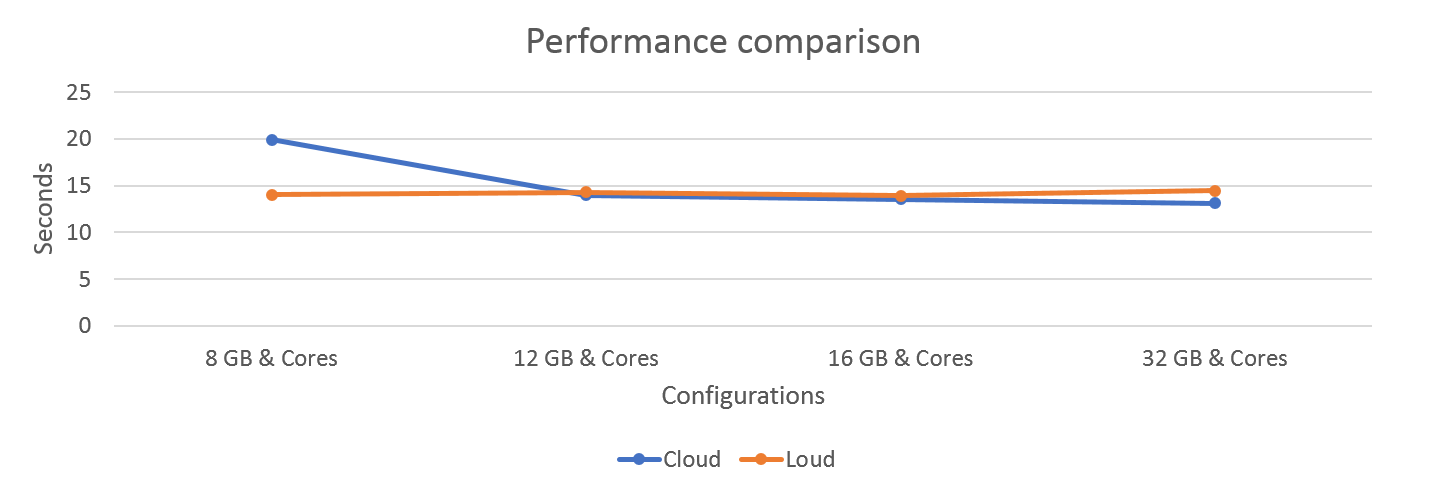
\includegraphics[width=\textwidth]{images/performance_comparison.png}
\textsuperscript{Figure 4.1.2 Performance comparison Cloud machines and physical devices}
\end{figure}

This shows that there is one big performance difference with the 8GB and 8 core devices. With this configuration the Cloud devices needed a bit less than 20 seconds, while the physical devices needed only round about 15 seconds. After that the performance of the physical devices doesn't increases any more, while the performance of the Cloud devices increases step by step. First for 12GB and 12 cores there has been a significant change, after it only small improvements.